% ============================================================
%  SECCIÓN 1: INTRODUCCIÓN
% ============================================================
\section{Introducción}

El aeropéndulo es una de las plataformas experimentales más interesantes en el ámbito de la teoría de control, debido a que el sistema exhibe un comportamiento dinámico no lineal y su susceptibilidad ante perturbaciones externas y dinámicas no modeladas.

\begin{figure}[ht]
    \centering
    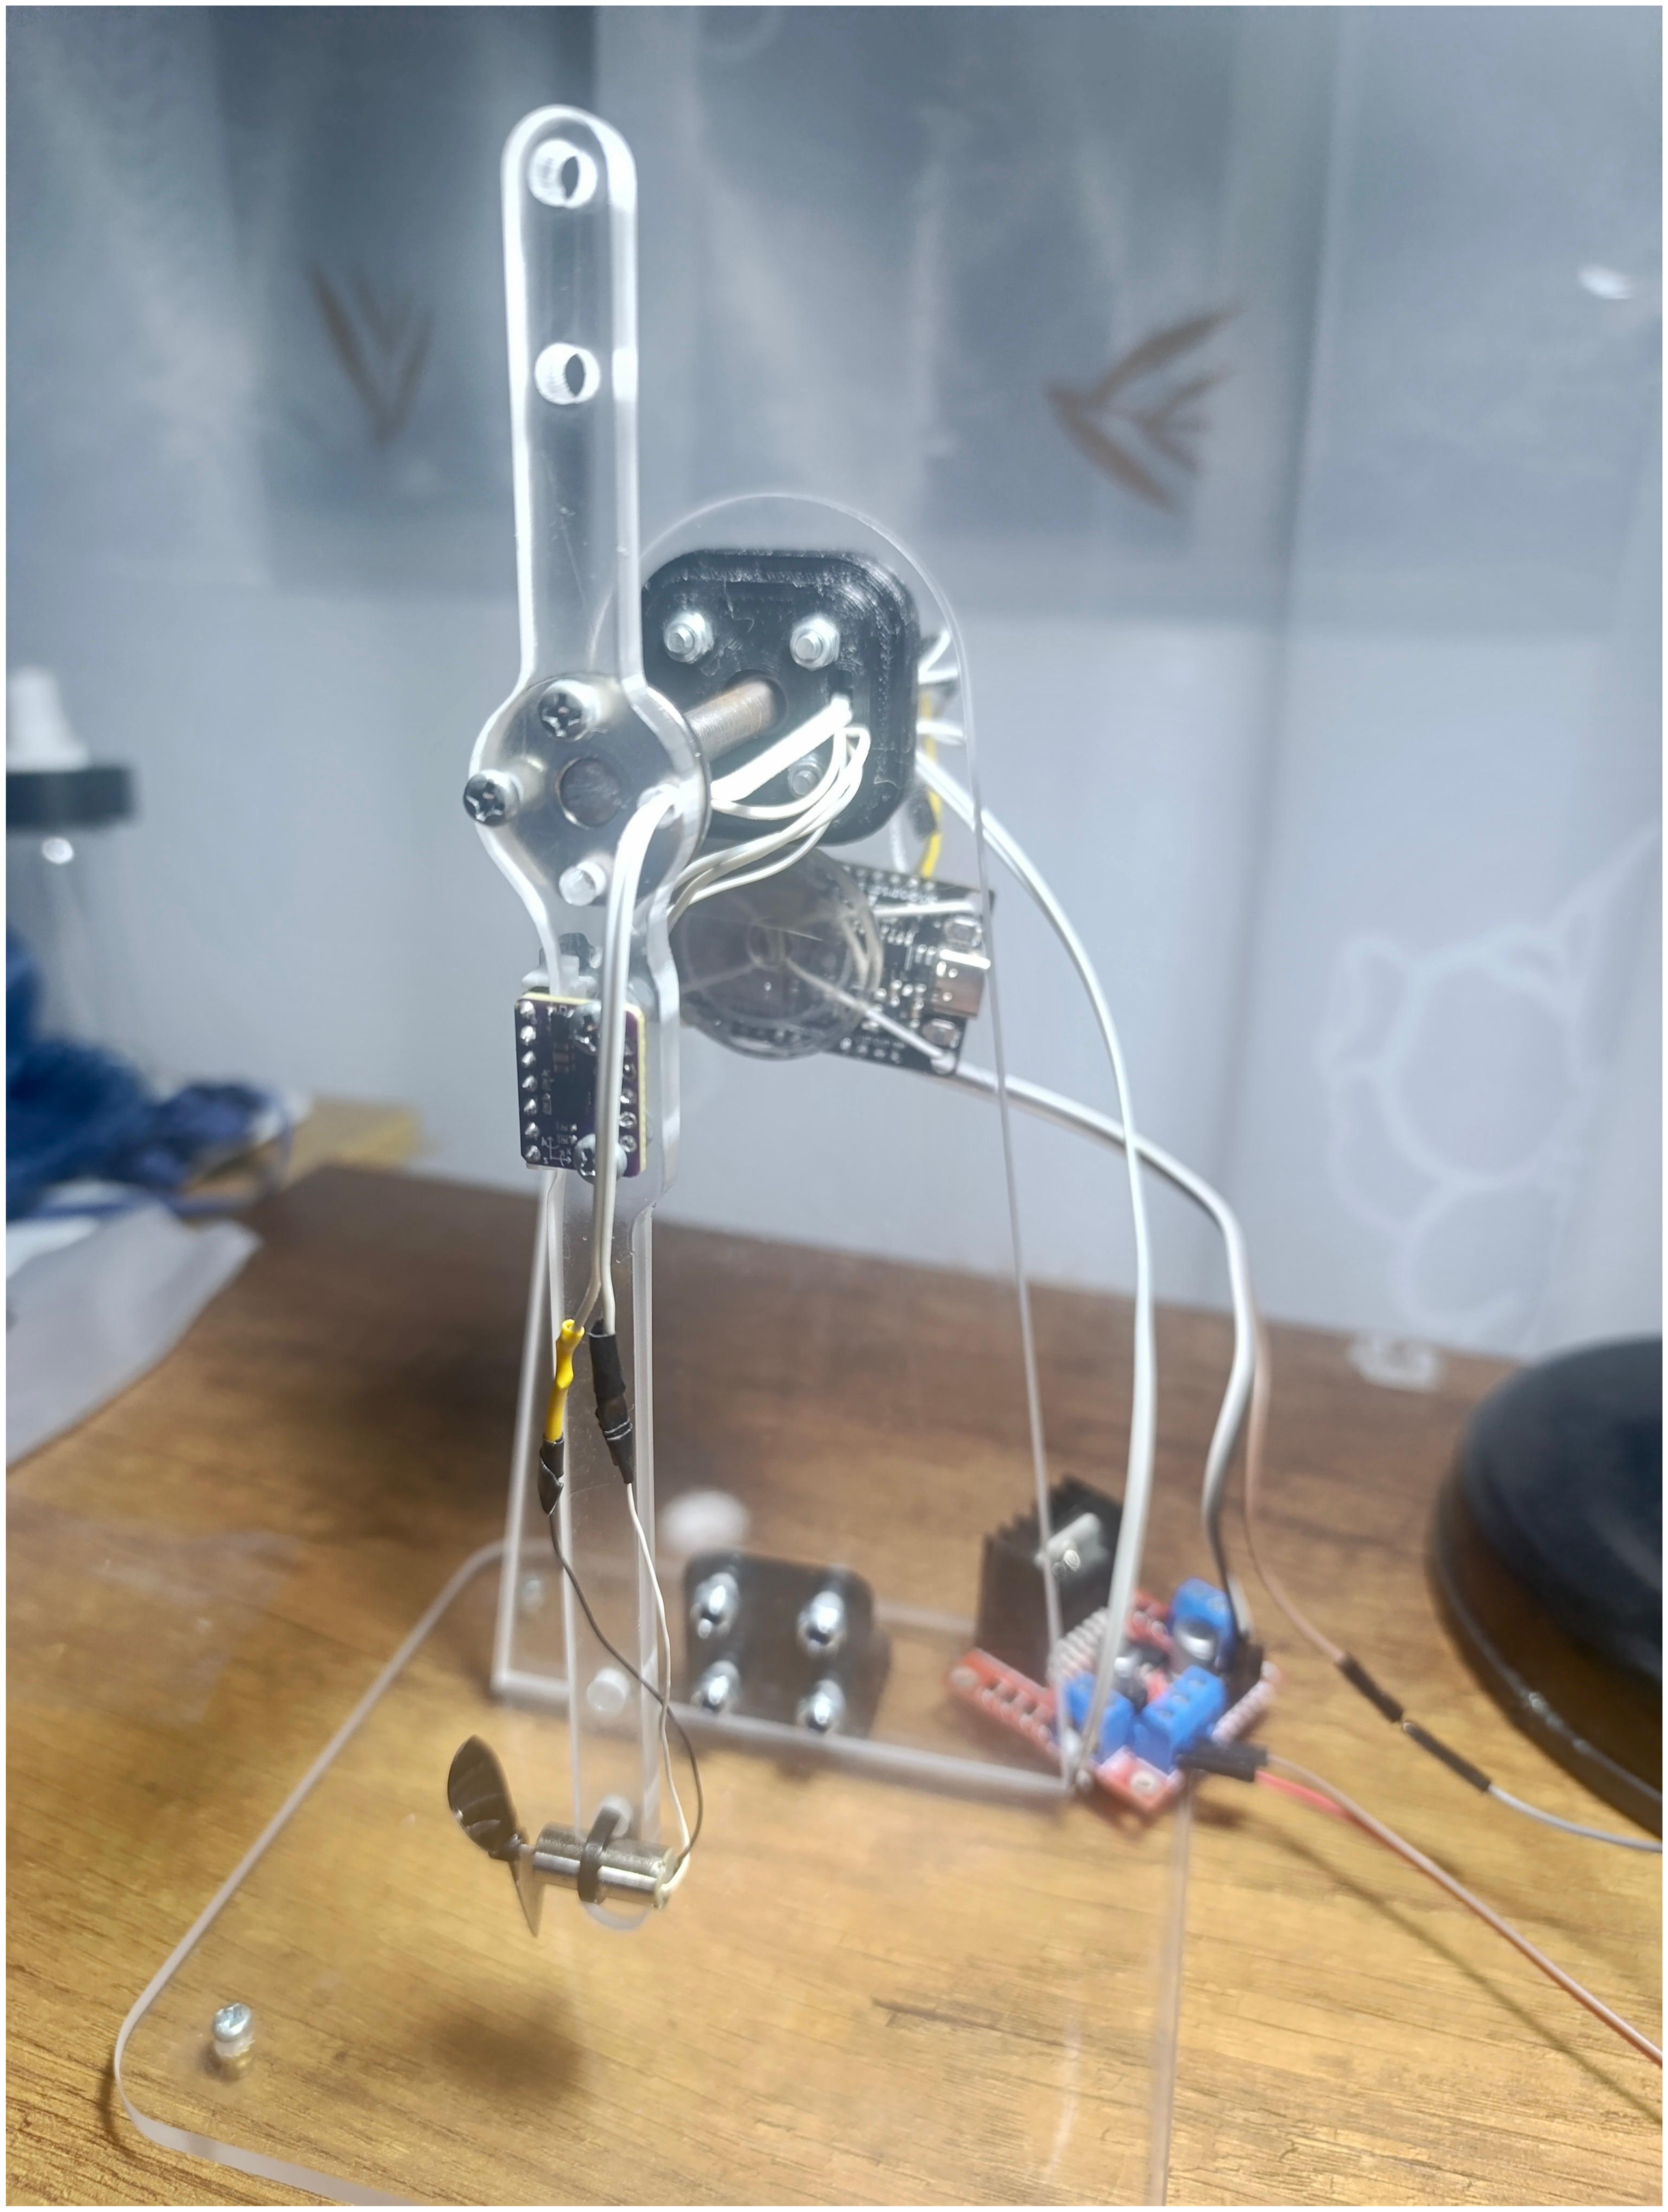
\includegraphics[width=0.3\textwidth]{Informe/Imagenes/planta.eps}
    \caption{Montaje del aeropéndulo}
    \label{fig:planta}
\end{figure}

El objetivo general de este proyecto es abordar el ciclo completo de ingeniería de control sobre un prototipo diseñado por nosotros mismo:
\begin{itemize}
  \item \textbf{Diseño e Integración Electromecánica:} Uso de procesos de manufactura rápida (corte láser e impresión 3D), un eje soportado por rodamientos y sensores controlados por un microcontrolador ESP32.
  
  \item \textbf{Caracterización Experimental de Parámetros:} Estimación de la ganancia del actuador ($K_{uf}$) y el coeficiente de fricción viscosa ($B$).
\end{itemize}
